\section{Conditional ice and geographic coastal alternatives}

\subsection{Carbon constraints beyond atmospheric concentration}
Atmospheric concentration alone does not identify terrestrial fertilization and
ocean transport separately. We prescribe the observed temperature history and
fit fertilization against NOAA CO$_2$ in 1979--2005, retaining 2006--2021 as a
holdout. The nine conditional fits vary respiration $Q_{10}=1,2,3$ and
mixed-layer exchange $\eta=10,16.87,30$\,m\,yr$^{-1}$. A bounded scalar search
over $\beta\in[0,2]$ is a new numerical experiment, not the wide R08 Bayesian
prior. Every fit begins in 1850 at the alternative closure's 280\,ppm equilibrium.
This avoids the missing pre-1850 land-use series but omits earlier perturbations.

Figure~\ref{fig:carbonfit} shows that fits with similar atmospheric residuals
predict different ocean inventories. At $Q_{10}=2$ and $\eta=16.87$\,m\,yr$^{-1}$,
the fitted $\beta=0.6680$ yields a 0.535\,ppm holdout RMSE and 118.06\,Gt\,C
ocean uptake by 1994. R08 cites the independent estimate $118\pm19$\,Gt\,C;
its nominal 1800--1994 interval differs from our 1850 initialization, as in
R08's equilibrium approximation. Predicted 1980s and 1990s ocean fluxes are
1.98 and 2.32\,Gt\,C\,yr$^{-1}$, compared with the written constraints
$1.6\pm0.4$ and $2.0\pm0.4$. These checks do not condition the fit.
Across all nine cases, time-step doubling changes CO$_2$ by at most
0.000333\,ppm and carbon accounting closes within $7\times10^{-12}$\,Gt\,C.
The remaining chemistry-version and prior uncertainties prevent interpreting
these conditional fits as the target carbon posterior.

\begin{figure}[htbp]
\centering\includegraphics[width=\textwidth]{carbon_conditional.pdf}
\caption{Conditional carbon alternatives. Left: fitted concentration histories
for three respiration choices at a fixed transfer rate; the vertical line ends
the fit. Centre: held-out concentration errors. Right: independently predicted
ocean inventory, with the observational interval cited by R08. The latter was
not used in optimization. These fits are not target-model reproductions.}
\label{fig:carbonfit}
\end{figure}

\subsection{Independent ice observations and identifiable parameters}
Independent IMBIE and GlaMBIE observations allow a conditional test of the
documented Greenland and glacier equations\cite{imbie,glambie}. IMBIE monthly
mass-change rates are averaged annually. Their errors are temporally dependent;
we use the arithmetic mean of monthly standard deviations as an upper bound on
annual-mean uncertainty, rather than dividing by $\sqrt{12}$. GlaMBIE supplies
annual rates and standard errors directly. All rates remain in Gt\,yr$^{-1}$
until the explicit conversion $362500$\,Gt per metre of sea-level equivalent.
Observed HadCRUT4 temperature is prescribed, so held-out ice years are a
conditional hindcast, not a forecast made without knowledge of temperature.

The glacier equation is separable. For $n\ne1$, define
$u=(1-S/V)^{1-n}$. Then
\begin{equation}
 u(t+\Delta t)=u(t)-\frac{(1-n)\beta}{V}
 \int_t^{t+\Delta t}[T(s)+0.15]\,\mathrm ds.
\end{equation}
The integral is exact for linearly interpolated annual temperature. For $n=1$
the remaining volume decays exponentially with the same temperature integral.
Zero remaining volume is absorbing, including extinction before the end of an
interval whose temperature later falls. This explicit convention resolves the
nonunique mathematical continuation for $n<1$.

For Greenland, write sea-level contribution $S=V_0-V$ and use the documented
linear equilibrium volume. The equation becomes
\begin{equation}
 \dot S=[d+kT-S]10^{-3}(aT+b),\qquad d=V_0-b_{\rm eq},\quad k=-c.
\end{equation}
Annual rates cannot distinguish $V_0$ and $b_{\rm eq}$ separately. Their B17
independent uniform priors induce a trapezoid density for $d$, which we derive
from the overlap of the two intervals. We retain that density instead of
inventing a uniform prior on the difference. Negative inverse response times
are excluded on the modeled temperature domain. Four RK4 steps per year agree
with refined and analytical cases.

We fit rates through 2014 and reserve 2015--2020. Glacier initialization in
1990 and Greenland initialization in 1961 are explicit alternatives. Physical
bounds follow B17; residual innovation standard deviation is newly assigned
$[0.1,250]$\,Gt\,yr$^{-1}$ and AR1 correlation $[0,0.999]$. These rate-error
priors differ from the original cumulative-state calibration. The first chains
failed the tail effective-sample criterion and were retained as failed attempts.
Only chains passing the recorded diagnostics enter subsequent projections.

The longer runs pass: the maximum $\widehat R$ is 1.0012 and the minimum
tail effective sample size exceeds 1100. Conditional holdout RMSE is
84.8\,Gt\,yr$^{-1}$ for glaciers and 128.9\,Gt\,yr$^{-1}$ for Greenland.
Both 90\% predictive intervals cover all six held-out years, but that short
record does not establish predictive accuracy. A straight-line glacier trend
fitted only to training data has lower holdout RMSE, 73.6\,Gt\,yr$^{-1}$.
The glacier model therefore does not improve on this simple baseline despite
its physical structure and converged sampler. Greenland improves on the tested
training-mean, last-year and linear-trend baselines (144--161\,Gt\,yr$^{-1}$).

Future component calculations pair complete ice-parameter rows with complete
joint climate rows independently. They do not recover the target's cross-model
posterior correlations. Integration restarts from the observed-temperature
hindcast state in 2021; its boundary temperature is observed, followed by modeled
temperatures on the same reference datum. Future ribbons include parameter
uncertainty only. The 0--2000\,m thermal component uses the independently fitted
NOAA coefficient, excluding unobserved deeper expansion.

\begin{figure}[htbp]
\centering\includegraphics[width=\textwidth]{ice_alternative.pdf}
\caption{Conditional ice-component alternatives. Upper panels compare annual
mass-loss rates with independent observations; the fit ends in 2014. Blue
ribbons show parameter uncertainty, orange ribbons held-out predictive
uncertainty including AR1 residuals and observational error. Lower panels show
parameter-only projections relative to 2010 for three SSP forcing scenarios.
These are separate component predictions, not a reproduced global sea-level
distribution.}
\label{fig:icealt}
\end{figure}

IMBIE gravimetry can contain peripheral glaciers also represented by GlaMBIE.
Combining these series without an overlap correction could double count ice
loss. The original component experiment therefore reports them separately.
Otosaka and coauthors\cite{imbie} quantify a4.1\%/3.3\% change in reconciled
Greenland/Antarctic estimates when peripheral glaciers are removed from
gravimetry over2002--2020, below reported uncertainty. This is a specific
accounting limitation, rather than a prohibition on any alternative total.
An explicitly uncorrected component budget and covariance sensitivities can
therefore be investigated, while exact target component boundaries and joint
calibration remain unresolved.

\subsection{Geographic exposure and regional accounting}
SLIIDERS v1.1 supplies independently published elevation-binned land, population,
capital, wetland, surge and socioeconomic inputs\cite{sliiders}. Only its input
product was retrieved; no pyCIAM implementation, construction scripts or model
outputs were consulted. Aggregating 11980 subadministrative records by coast
and country yields 9574 groups. Six have no coastline and 37 lack positive
economic inputs; their inventories and exclusion reasons remain in a separate
CSV. The experiment uses the remaining 9531 coast-country groups.

The alternative uses SSP2 and SSP4 OECD economics in 2019 USD PPP, annual
interpolation between decadal nodes, and a 2010--2100 horizon. Sea level is
spatially uniform and prescribed as $h[(t-2010)/90]^{1.5}$, with $h=0.5,1,2$\,m.
It has no temperature-conditioned probability interpretation. The model selects
the least-cost first-period policy, retains its strategy and return level, and
updates height or retreat thresholds in 2051. Costs are discounted to 2010 at
4\%. Incremental cost subtracts a paired zero-SLR calculation. The lowest
retreat level follows mean sea level, an explicit alternative to unavailable
DINAS annual-high-tide inputs. Wetland exposure follows its actual elevation
profile, with the documented rate-dependent loss fraction. These conventions
do not recover the target's segmentation, monetary basis, decadal accounting,
2150 horizon or spatial fingerprints.

The initial pilot exposed a 9.0\% quadrature discrepancy in no-adaptation costs:
narrow surge densities could lie between nodes even when elevation breaks
were resolved. Splitting integration at both elevation breaks and hazard
quantiles reduces the maximum 12-versus-24-node difference to
$1.5\times10^{-11}$ across 114 pilot cases, with no policy changes. Original
0.1\,m profiles additionally test the separate six-bin exposure approximation.
Numerical integration agreement does not validate exposure coarsening.
Indeed, original-resolution profiles change two of the 114 pilot policy choices
and increase summed incremental cost by 9.6\%. The largest individual relative
change is 71.6\%. This deterministic pilot is not representative sampling and
cannot supply a global correction factor. The coarse global experiment remains
a sensitivity result while a full original-resolution SSP4, 1\,m calculation
tests the global effect.

Regional ratios use independent World Bank national GDP\cite{worldbank}.
We value 2010 GDP at 2019 PPP by multiplying 2019 current-PPP GDP by the
country's 2010/2019 real-GDP ratio. Available landlocked-country GDP is included
in denominators; coastal costs lacking a matching positive GDP are excluded
from the ratios and their coverage is recorded. Afghanistan and Pakistan are
restored to their pre-July-2025 South Asia classification, as documented by the
World Bank. These explicit choices support an inequality sensitivity experiment,
not reproduction of the target's regional numerical bars.

\begin{figure}[htbp]
\centering\includegraphics[width=\textwidth]{geographic_alternative.pdf}
\caption{Geographic coastal alternatives. Upper left: global incremental costs
for prescribed uniform sea-level paths, with paired no-SLR baselines for both
selected policy and no adaptation. Upper right: unadjusted cost components for
SSP4 and 1\,m. Lower left: positive incremental costs at coast coordinates;
points represent input coast-country groups, not population density. Lower
right: regional minus global cost/GDP fractions at 1\,m using independent GDP
inputs and documented coverage exclusions. Every panel is a non-reproduction;
the paths have no calibrated warming-bin or tail probability.}
\label{fig:geoalt}
\end{figure}
\begin{table}[htbp]
\centering\small
\begin{tabular}{llrrr}
\toprule
SSP & Rise (m) & Selected cost & No-adapt. cost & Migrants (million) \\
\midrule
SSP2 & 0.5 & 0.435 & 11.824 & 99.465 \\
SSP2 & 1.0 & 1.019 & 25.776 & 127.280 \\
SSP2 & 2.0 & 2.370 & 57.592 & 197.987 \\
SSP4 & 0.5 & 0.421 & 10.131 & 98.755 \\
SSP4 & 1.0 & 0.990 & 22.141 & 125.951 \\
SSP4 & 2.0 & 2.305 & 50.112 & 195.002 \\
\bottomrule\end{tabular}
\caption{Geographic alternative totals. Cost columns are trillion 2019 USD PPP, discounted to2010. Migrants count movements in the selected policy over2010--2100 and are not unique individuals over a demographic lifetime. No warming probabilities are assigned.}
\end{table}
\begin{table}[htbp]
\centering\small
\begin{tabular}{lrrrr}
\toprule
Ice component & Max $\widehat R$ & Min bulk ESS & Min tail ESS & Holdout RMSE (Gt/yr) \\
\midrule
Glaciers & 1.0009 & 2752 & 1116 & 84.8 \\
Greenland & 1.0011 & 4449 & 2561 & 128.9 \\
\bottomrule\end{tabular}
\caption{Final conditional ice calibration diagnostics and held-out rate errors. Every coordinate and log density must pass $\widehat R<1.01$ and both ESS$\ge400$. Observed temperature is supplied in held-out years.}
\end{table}


\subsection{Complete original-resolution coastal comparison}
The earlier19-unit pilot cannot establish a global elevation-resolution error.
A subsequent paired experiment evaluates every eligible unit with all200
original0.1 m exposure bins, retaining the same inputs, prescribed trajectory,
quadrature and policy conventions. Figure\ref{fig:fullresolution} and the
computed table report the complete comparison. Its cost difference is an
effect of redistributing exposure within the original six bins, rather than
adding population, capital or land to the domain. Independent binary and CSV
readers agree exactly on the original-resolution pilot; doubled flood
quadrature changes costs by less than $2\times10^{-13}$ in relative terms
and changes no pilot policy.
\begin{figure}[htbp]
\centering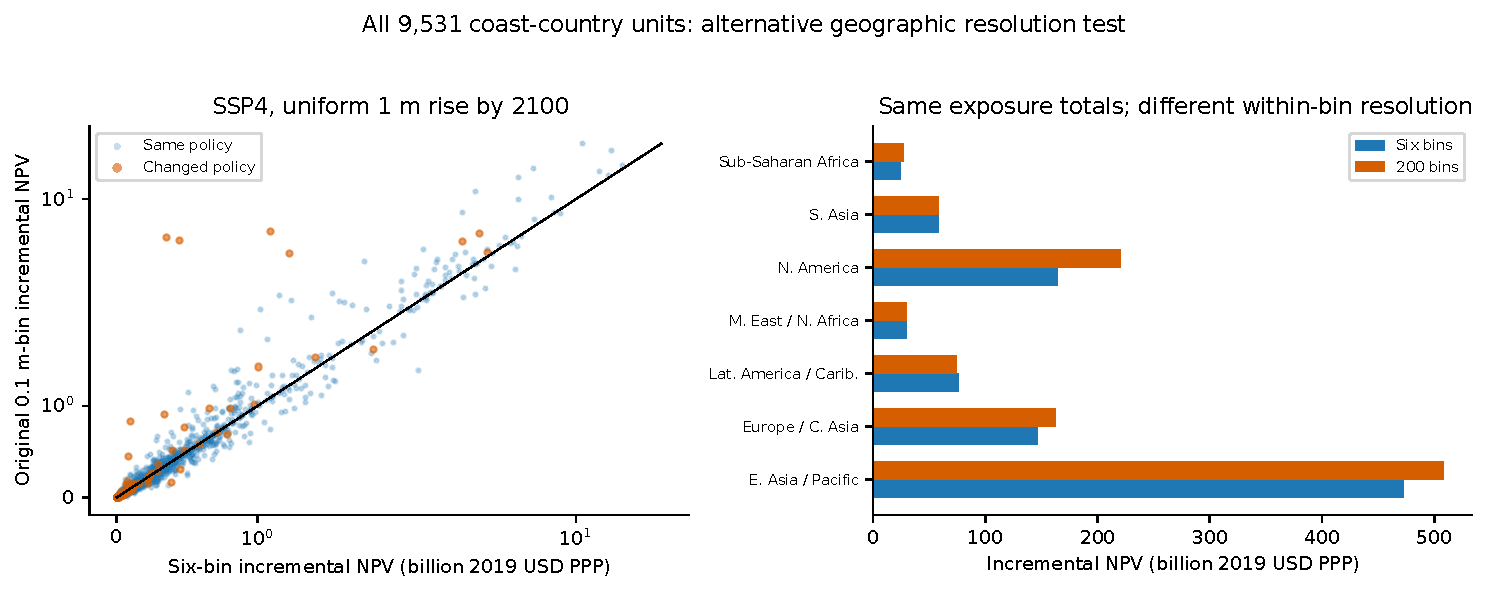
\includegraphics[width=\linewidth]{figures/geographic_full_resolution.pdf}
\caption{Matched SSP4,1 m coastal calculations for all9,531 eligible units.
Left: incremental cost after subtraction of the paired zero-rise baseline;
both axes use a symmetric logarithmic scale and the line marks equality.
Right: World Bank regional totals under the same two elevation resolutions.
Both calculations are geographic alternatives with uniform prescribed sea
level, annual2010--2100 cash flows, and2019 PPP values. They are not recovered
Wong warming-conditioned costs.}\label{fig:fullresolution}
\end{figure}
\begin{table}[htbp]
\centering\small
\begin{tabular}{lrrr}
\toprule
Quantity & Six bins & 200 bins & Change (\%) \\
\midrule
Selected policy total NPV & 2.9932 & 3.0576 & +2.15 \\
Paired-baseline incremental NPV & 0.9900 & 1.0992 & +11.03 \\
Movement count (million) & 125.9506 & 128.5904 & +2.10 \\
\bottomrule\end{tabular}
\caption{Complete matched resolution test for 9,531 coast-country units, SSP4 and prescribed1 m rise by2100. Cost rows use trillion 2019 USD PPP. The input elevation range is unchanged; only within-bin exposure resolution changes.}
\end{table}
The preferred first-period policy changes in 148 units (1.55\%). These totals replace extrapolation from the small coastal pilot; they do not establish convergence of the physical exposure data themselves.

